\documentclass[12pt,a4paper]{article}

\usepackage[utf8]{inputenc}
\usepackage[T1]{fontenc}
\usepackage[a4paper,margin=1in]{geometry}
\usepackage{hyperref}
\usepackage{xcolor}
\usepackage{listings}
\usepackage{longtable}
\usepackage{array}
\usepackage{enumitem}
\usepackage{pgfplots}

\pgfplotsset{compat=1.18}

\hypersetup{
    colorlinks=true,
    linkcolor=blue,
    urlcolor=blue
}

\definecolor{codebg}{RGB}{245,245,245}
\definecolor{codeframe}{RGB}{220,220,220}

\lstset{
    basicstyle=\ttfamily\small,
    backgroundcolor=\color{codebg},
    frame=single,
    rulecolor=\color{codeframe},
    breaklines=true,
    columns=fullflexible,
    keepspaces=true
}

\title{Phase 1 to Phase 7 Report\\Environment Setup, Firmware Skeleton, Virtual Sensor, Sampling Benchmark, Frequency Analysis, Adaptive Sampling, and Aggregate Computation}
\author{IoT Adaptive Sampling Project}
\date{April 2026}

\begin{document}

\maketitle

\section{Introduction}

This document reports the work completed in \textbf{Phase 1},
\textbf{Phase 2}, \textbf{Phase 3}, \textbf{Phase 4}, \textbf{Phase 5},
\textbf{Phase 6}, and \textbf{Phase 7} of the project.

The purpose of Phase 1 was not to implement the full IoT application yet, but
to verify that the development environment, the ESP32 board, and the MQTT
communication tools were working correctly.

The purpose of Phase 2 was to convert the initial project structure into a real
firmware skeleton that boots on the target board and clearly separates the main
modules of the final system.

The purpose of Phase 3 was to replace the placeholder input with a real virtual
signal generator and verify that complete sample windows could be collected and
validated on the board.

The purpose of Phase 4 was to measure the highest stable sampling rate that the
current firmware and board could sustain under a strict timing criterion.

The purpose of Phase 5 was to replace the frequency-analysis placeholder with a
real spectral computation so that the dominant component of the generated
signal could be identified from each completed window.

The purpose of Phase 6 was to use the detected dominant frequency to change the
sampling rate at runtime while keeping later windows clean and internally
consistent.

The purpose of Phase 7 was to convert each completed analysis window into a
real aggregate result so that the average value, current sampling rate, and
dominant frequency are available for later communication stages.

The main goal of these early phases was to answer the following practical
questions:

\begin{quote}
Can the hardware and software environment already support firmware upload,
serial monitoring, and MQTT communication before the real project logic is
implemented, can the project boot as a structured modular firmware before
the real sensing and FFT logic are added, can it generate the required virtual
signal, and what is the highest stable sampling rate observed in the current
implementation, and can the dominant spectral component be detected correctly
from the measured signal windows, and can the system safely adapt its sampling
rate based on that detected frequency, and can each completed window now
produce a clean aggregate summary for later transmission?
\end{quote}

These phases are important because they reduce technical risk. If the
environment and firmware structure are not validated first, later problems with
FFT, adaptive sampling, or network communication may be difficult to diagnose.

\section{Goal of Phase 1}

The objective of Phase 1 was to validate five basic requirements:

\begin{enumerate}[label=\arabic*.]
    \item the ESP32 board is detected by the computer,
    \item a simple firmware example can be built and uploaded,
    \item the serial monitor shows correct runtime logs,
    \item the MQTT broker is running correctly,
    \item MQTT communication works both locally and over the local network.
\end{enumerate}

If all five checks pass, the environment is considered ready for the next
development phase.

\section{Hardware and Software Used}

\subsection{Hardware}

The hardware used in this phase is:

\begin{itemize}
    \item \textbf{RUIZHI ESP32 V3 LoRa Board}
    \item USB connection to the development computer
    \item integrated WiFi interface
    \item integrated LoRa radio, not used yet in Phase 1
\end{itemize}

\subsection{Software}

The software and tools used in this phase are:

\begin{itemize}
    \item \textbf{PlatformIO} with the \texttt{ESP-IDF} framework
    \item \textbf{Mosquitto} as MQTT broker
    \item \textbf{PowerShell} on Windows
    \item serial monitor through PlatformIO
\end{itemize}

\subsection{Network Information}

The local network address used during testing was:

\begin{itemize}
    \item \textbf{Broker IP:} \texttt{192.168.1.22}
    \item \textbf{MQTT Port:} \texttt{1883}
\end{itemize}

\section{Smoke Test Project Created for Phase 1}

To keep the first test simple and reliable, a small smoke test project was
created. Its only purpose was to prove that firmware could be built, uploaded,
and executed successfully.

The test project uses:

\begin{itemize}
    \item PlatformIO project configuration for the board
    \item \texttt{ESP-IDF} as the framework
    \item a minimal \texttt{app\_main()} function
    \item repeated serial output and automatic restart
\end{itemize}

The board target used in the test project is:

\begin{lstlisting}
[env:heltec_wifi_lora_32_V3]
platform = espressif32
framework = espidf
board = heltec_wifi_lora_32_V3
monitor_speed = 115200
\end{lstlisting}

This configuration was chosen because it matches the ESP32-S3 based Heltec
compatible board used in the project.

\section{Detailed Step-by-Step Procedure}

\subsection{Step 1: Detect the ESP32 Board}

The first step was to verify whether Windows could correctly detect the board
when it was connected through USB.

\subsubsection*{Why this step matters}

If the operating system does not detect the board correctly, then firmware
upload and serial monitoring cannot work.

\subsubsection*{What was checked}

The connected serial devices were inspected in Windows. The relevant result was:

\begin{itemize}
    \item \texttt{COM3} was detected as \texttt{Silicon Labs CP210x USB to UART Bridge}
\end{itemize}

\subsubsection*{Interpretation}

This result confirms that the ESP32 development board is visible to the
computer and that the USB-to-serial interface driver is working correctly.

\subsubsection*{Result}

\textbf{Status: Passed}

\subsection{Step 2: Build a Minimal Firmware Example}

After confirming the board was detected, the next step was to build a very
small firmware application.

\subsubsection*{Why this step matters}

This step validates:

\begin{itemize}
    \item the compiler toolchain,
    \item the board definition,
    \item the ESP-IDF integration,
    \item the project configuration.
\end{itemize}

\subsubsection*{What was implemented}

A simple firmware program was created with the following behavior:

\begin{itemize}
    \item print a greeting message,
    \item print chip information,
    \item print free heap memory,
    \item count down from 5 seconds,
    \item restart automatically.
\end{itemize}

\subsubsection*{Key command used}

\begin{lstlisting}
& "$HOME\.platformio\penv\Scripts\pio.exe" run
\end{lstlisting}

\subsubsection*{Interpretation}

The successful build showed that the local PlatformIO and ESP-IDF environment
were correctly set up for this board.

\subsubsection*{Result}

\textbf{Status: Passed}

\subsection{Step 3: Upload the Firmware to the Board}

Once the project compiled successfully, the firmware was uploaded to the board.

\subsubsection*{Why this step matters}

Successful upload proves that:

\begin{itemize}
    \item the correct serial port is selected,
    \item the bootloader flashing process works,
    \item the board can accept new firmware.
\end{itemize}

\subsubsection*{Key command used}

\begin{lstlisting}
& "$HOME\.platformio\penv\Scripts\pio.exe" run -t upload --upload-port COM3
\end{lstlisting}

\subsubsection*{Interpretation}

Since the test firmware ran correctly after flashing, the upload process was
successful.

\subsubsection*{Result}

\textbf{Status: Passed}

\subsection{Step 4: Verify Runtime Through the Serial Monitor}

After uploading, the serial monitor was opened to confirm that the board was
actually running the expected program.

\subsubsection*{Why this step matters}

This step confirms:

\begin{itemize}
    \item the board boots correctly,
    \item the uploaded application starts correctly,
    \item runtime logs can be observed,
    \item future debugging will be possible.
\end{itemize}

\subsubsection*{Observed output}

The following output was observed:

\begin{lstlisting}
Hello world from Stage 1!
This is esp32s3 with 2 CPU core(s), WiFi/BLE, silicon revision v0.2,
8MB external flash
Minimum free heap size: 388752 bytes
Stage 1 smoke test restart in 5 seconds...
Stage 1 smoke test restart in 4 seconds...
Stage 1 smoke test restart in 3 seconds...
Stage 1 smoke test restart in 2 seconds...
Stage 1 smoke test restart in 1 seconds...
Stage 1 smoke test restart in 0 seconds...
Restarting now.
\end{lstlisting}

Additional boot logs also showed:

\begin{itemize}
    \item target chip: \texttt{esp32s3}
    \item flash size: \texttt{8MB}
    \item ESP-IDF version: \texttt{5.5.3}
\end{itemize}

\subsubsection*{Interpretation}

This output confirms that:

\begin{itemize}
    \item the firmware was uploaded correctly,
    \item the application executed correctly,
    \item the serial monitor configuration was correct,
    \item the board information was consistent with the expected hardware.
\end{itemize}

\subsubsection*{Result}

\textbf{Status: Passed}

\subsection{Step 5: Start the MQTT Broker}

The next objective was to verify the MQTT side of the environment.

\subsubsection*{Why this step matters}

The project requires sending aggregate values from the ESP32 to a nearby edge
server using MQTT over WiFi. Before implementing this in firmware, the broker
must be available and working.

\subsubsection*{Initial command used}

\begin{lstlisting}
& "C:\Program Files\mosquitto\mosquitto.exe" -v
\end{lstlisting}

\subsubsection*{Initial result}

The broker did not start in that terminal because port \texttt{1883} was
already in use.

\subsubsection*{Interpretation}

This was not a real failure. It meant that a Mosquitto instance was already
running on the machine. Further inspection showed that Mosquitto was already
installed and active as a Windows service.

\subsubsection*{Result}

\textbf{Status: Passed}

\subsection{Step 6: Verify Local MQTT Publish/Subscribe}

After confirming that Mosquitto was already running, the broker was tested
locally on the same machine.

\subsubsection*{Why this step matters}

This verifies that the broker is operational and can route MQTT messages
correctly between a publisher and a subscriber.

\subsubsection*{Commands used}

Subscriber:

\begin{lstlisting}
& "C:\Program Files\mosquitto\mosquitto_sub.exe" -h localhost -t stage1/test -v
\end{lstlisting}

Publisher:

\begin{lstlisting}
& "C:\Program Files\mosquitto\mosquitto_pub.exe" -h localhost -t stage1/test -m "hello from stage1"
\end{lstlisting}

\subsubsection*{Observed result}

\begin{lstlisting}
stage1/test hello from stage1
\end{lstlisting}

\subsubsection*{Interpretation}

This result proves that:

\begin{itemize}
    \item the broker is alive,
    \item a client can subscribe to a topic,
    \item another client can publish to the same topic,
    \item the broker routes the message correctly.
\end{itemize}

\subsubsection*{Result}

\textbf{Status: Passed}

\subsection{Step 7: Make MQTT Reachable Over the Local Network}

At this point, MQTT worked only on \texttt{localhost}. However, the real
project requires the ESP32 board to connect over WiFi using the local network.

\subsubsection*{Why this step matters}

If Mosquitto only listens on \texttt{localhost}, then the development computer
can use it, but the ESP32 cannot reach it over WiFi.

\subsubsection*{Problem observed}

Mosquitto was running in \textit{local only mode}. This means it accepted
connections only from the local machine.

\subsubsection*{Configuration change applied}

The broker configuration file was updated so that Mosquitto listens on all IPv4
interfaces:

\begin{lstlisting}
listener 1883 0.0.0.0
protocol mqtt
socket_domain ipv4
listener_allow_anonymous true
\end{lstlisting}

\subsubsection*{Additional note}

The service restart required administrative privileges, and it was also
necessary to ensure the configuration lines were not commented out.

\subsubsection*{Interpretation}

This change made the broker visible not only to the local machine, but also to
devices on the same local network, including the ESP32 board.

\subsection{Step 8: Verify MQTT Over LAN}

The final Phase 1 check was to verify MQTT communication using the LAN address
of the development computer instead of \texttt{localhost}.

\subsubsection*{Why this step matters}

This test is the closest software-side approximation to the future ESP32
communication scenario.

\subsubsection*{Commands used}

Subscriber:

\begin{lstlisting}
& "C:\Program Files\mosquitto\mosquitto_sub.exe" -h 192.168.1.22 -t stage1/test -v
\end{lstlisting}

Publisher:

\begin{lstlisting}
& "C:\Program Files\mosquitto\mosquitto_pub.exe" -h 192.168.1.22 -t stage1/test -m "hello over lan"
\end{lstlisting}

\subsubsection*{Observed result}

\begin{lstlisting}
stage1/test hello over lan
\end{lstlisting}

\subsubsection*{Interpretation}

This confirms that:

\begin{itemize}
    \item the broker is listening on the LAN,
    \item the chosen port is correct,
    \item the network path is working,
    \item the ESP32 will later be able to use the same broker address from
    firmware.
\end{itemize}

\subsubsection*{Result}

\textbf{Status: Passed}

\section{Problems Encountered and How They Were Solved}

During Phase 1, a few small setup issues appeared. They were useful because
they helped confirm the behavior of the system.

\subsection{Problem 1: Port 1883 Already in Use}

\textbf{Observation:} when Mosquitto was started manually, it reported that
port \texttt{1883} was already in use.

\textbf{Cause:} Mosquitto was already running as a Windows service.

\textbf{Solution:} instead of starting a second broker, the existing service
was used.

\subsection{Problem 2: Service Restart Failed}

\textbf{Observation:} restarting the service from PowerShell failed.

\textbf{Cause:} administrative privileges were required.

\textbf{Solution:} the restart had to be performed from an Administrator
PowerShell or from the Windows services panel.

\subsection{Problem 3: Listener Configuration Did Not Take Effect}

\textbf{Observation:} the broker remained local-only after editing the config.

\textbf{Cause:} the new configuration lines were still commented out with the
\texttt{\#} character.

\textbf{Solution:} the comment characters were removed and the service was
restarted.

\section{Summary of Phase 1 Results}

\begin{longtable}{|>{\raggedright\arraybackslash}p{0.60\textwidth}|>{\raggedright\arraybackslash}p{0.22\textwidth}|}
\hline
\textbf{Check} & \textbf{Status} \\
\hline
ESP32 board detected by Windows on COM3 & Passed \\
\hline
Minimal firmware built successfully & Passed \\
\hline
Firmware uploaded successfully & Passed \\
\hline
Serial monitor showed correct runtime logs & Passed \\
\hline
Mosquitto broker available on the computer & Passed \\
\hline
MQTT publish/subscribe worked on localhost & Passed \\
\hline
MQTT publish/subscribe worked over LAN IP \texttt{192.168.1.22} & Passed \\
\hline
\end{longtable}

\section{Phase 2: Firmware Skeleton}

\subsection{Goal of Phase 2}

The goal of Phase 2 was to build the first real version of the firmware
architecture for the project.

At this stage, the objective was still not to implement the final sensing
logic. Instead, the purpose was to create a clean and testable application
structure with separate modules and FreeRTOS tasks.

In practical terms, Phase 2 had to answer this question:

\begin{quote}
Can the firmware boot as a modular application on the ESP32 board, with all
planned subsystems initialized and running as placeholder tasks?
\end{quote}

\subsection{Expected Result of Phase 2}

Phase 2 was considered complete if the following conditions were satisfied:

\begin{enumerate}[label=\arabic*.]
    \item the firmware project compiles successfully,
    \item the application boots correctly on the ESP32 board,
    \item the modules are separated into their own source files,
    \item the FreeRTOS tasks are created correctly,
    \item startup logs confirm that all modules are initialized,
    \item a supervisor log confirms that the complete structure is active.
\end{enumerate}

\subsection{Project Structure Implemented}

The firmware project was created under the directory:

\begin{itemize}
    \item \texttt{firmware/esp32\_node}
\end{itemize}

The Phase 2 implementation included:

\begin{itemize}
    \item a PlatformIO configuration file,
    \item top-level ESP-IDF CMake files,
    \item shared project configuration,
    \item shared project data types,
    \item one source module for each planned subsystem,
    \item a central \texttt{app\_main()} entry point.
\end{itemize}

The firmware modules created in this phase are:

\begin{itemize}
    \item signal input
    \item signal processing
    \item sampling control
    \item MQTT communication
    \item LoRaWAN communication
    \item metrics
    \item display
\end{itemize}

\subsection{Why This Structure Was Chosen}

The final project will contain multiple responsibilities:

\begin{itemize}
    \item sample acquisition
    \item FFT-based analysis
    \item adaptive sampling control
    \item MQTT transmission
    \item LoRaWAN transmission
    \item measurement collection
    \item optional display output
\end{itemize}

Putting all of these responsibilities into a single file would make the code
harder to maintain and harder to debug.

For this reason, the firmware was divided into modules from the beginning. This
allows future phases to add real logic without changing the overall
architecture.

\subsection{Shared Data Structures Created}

To allow the modules to communicate with each other, shared structures were
defined in the common project headers.

The most important data structures introduced in Phase 2 are:

\begin{itemize}
    \item \texttt{raw\_sample\_t}
    \item \texttt{fft\_result\_t}
    \item \texttt{aggregate\_result\_t}
    \item \texttt{transmission\_payload\_t}
    \item \texttt{timing\_metrics\_t}
    \item \texttt{project\_context\_t}
\end{itemize}

\subsubsection*{Purpose of each structure}

\begin{itemize}
    \item \texttt{raw\_sample\_t}: stores one generated or measured sample
    together with timestamp and source information.
    \item \texttt{fft\_result\_t}: stores the dominant frequency result for one
    signal window.
    \item \texttt{aggregate\_result\_t}: stores the average and metadata for a
    completed window.
    \item \texttt{transmission\_payload\_t}: stores prepared payloads for MQTT
    or LoRaWAN communication.
    \item \texttt{timing\_metrics\_t}: stores counters and timestamps useful for
    system measurement.
    \item \texttt{project\_context\_t}: contains the queues, event group, mode,
    and shared metrics of the whole application.
\end{itemize}

\subsection{FreeRTOS Communication Model}

Phase 2 also introduced the basic communication model between tasks.

The following FreeRTOS objects were created:

\begin{itemize}
    \item sample queue
    \item FFT queue
    \item aggregate queue
    \item MQTT queue
    \item LoRaWAN queue
    \item one event group for module readiness flags
\end{itemize}

\subsubsection*{Why queues were chosen}

Queues were selected because they provide a clean and safe way to pass data
between tasks. They are especially suitable for this project because the final
system naturally has a pipeline:

\begin{enumerate}[label=\arabic*.]
    \item generate or read samples,
    \item process a signal window,
    \item adapt the sampling logic,
    \item prepare communication payloads,
    \item transmit results.
\end{enumerate}

This makes queues a natural fit for the project design.

\subsubsection*{Why event groups were chosen}

The event group was introduced to track whether each subsystem had initialized
correctly. This makes the startup process easier to observe and later makes it
possible to add stronger supervision logic if needed.

\subsection{Main Firmware Entry Point}

The central application entry point was implemented in \texttt{app\_main()}.

The responsibilities of \texttt{app\_main()} in Phase 2 are:

\begin{itemize}
    \item print startup information,
    \item create the shared project context,
    \item create the FreeRTOS queues,
    \item create the event group,
    \item initialize every module,
    \item create one task per module,
    \item print a periodic supervisor heartbeat.
\end{itemize}

\subsection{Placeholder Behavior Implemented in Each Module}

At this phase, each module contains only placeholder logic. This is
intentional. The goal is to prove that the architecture works before adding
real sensing and processing.

\subsubsection{Signal Input Module}

The signal input module currently:

\begin{itemize}
    \item initializes correctly,
    \item sets its ready flag,
    \item periodically creates a placeholder sample,
    \item pushes the sample into the sample queue.
\end{itemize}

The placeholder sample currently has:

\begin{itemize}
    \item source = virtual sensor
    \item value = 0.0
    \item a valid sample id
    \item a real timestamp
\end{itemize}

\subsubsection{Signal Processing Module}

The signal processing module currently:

\begin{itemize}
    \item receives placeholder samples from the sample queue,
    \item logs that it received them,
    \item creates a placeholder FFT result every four samples,
    \item sends that result to the FFT queue.
\end{itemize}

No real FFT is performed yet. That work belongs to a later phase.

\subsubsection{Sampling Control Module}

The sampling control module currently:

\begin{itemize}
    \item waits for FFT results,
    \item logs a placeholder adaptive decision,
    \item confirms that the control stage is wired correctly.
\end{itemize}

No real adaptive policy is applied yet.

\subsubsection{MQTT Module}

The MQTT module currently:

\begin{itemize}
    \item initializes with the configured broker address,
    \item prepares placeholder JSON messages,
    \item pushes them into the MQTT queue,
    \item logs the prepared payload.
\end{itemize}

At this phase it does not yet open a WiFi or broker connection.

\subsubsection{LoRaWAN Module}

The LoRaWAN module currently:

\begin{itemize}
    \item initializes correctly,
    \item prepares a placeholder uplink payload,
    \item pushes it into the LoRaWAN queue,
    \item logs the operation.
\end{itemize}

No real TTN communication is implemented yet.

\subsubsection{Metrics Module}

The metrics module currently:

\begin{itemize}
    \item initializes the shared timing structure,
    \item updates counters and timestamps,
    \item prints periodic metrics heartbeats.
\end{itemize}

\subsubsection{Display Module}

The display module currently:

\begin{itemize}
    \item initializes correctly,
    \item logs a periodic heartbeat,
    \item confirms that the display subsystem is included in the architecture.
\end{itemize}

In Phase 2 it is only a serial placeholder and does not yet use the OLED.

\subsection{Build Validation}

After implementing the firmware skeleton, the project was compiled locally.

\subsubsection*{Why this step matters}

This build validation confirms:

\begin{itemize}
    \item the project structure is correct,
    \item the headers and components are connected correctly,
    \item the application is syntactically valid,
    \item the firmware can be built for the target board.
\end{itemize}

\subsubsection*{Result}

The firmware built successfully using PlatformIO and the ESP-IDF framework.

An additional configuration improvement was made during this phase:

\begin{itemize}
    \item the flash size configuration was updated from \texttt{2MB} to
    \texttt{8MB} so that it matches the actual board hardware.
\end{itemize}

\subsection{Runtime Validation on the Board}

After compiling the firmware, it was uploaded to the ESP32 and observed through
the serial monitor.

\subsubsection*{Why this step matters}

This is the most important validation of Phase 2 because it proves that the
modular application does not only compile, but also runs correctly on the
actual board.

\subsubsection*{Observed startup log}

The runtime log showed the following important lines:

\begin{lstlisting}
I (...) app_main: Phase 2 firmware skeleton booting for adaptive-sampling-node
I (...) app_main: Planned MQTT endpoint: 192.168.1.22:1883
I (...) metrics: Metrics module initialized
I (...) signal_input: Signal input module ready in placeholder mode
I (...) signal_processing: Signal processing module ready with FFT placeholder hooks
I (...) sampling_control: Sampling control module ready with adaptive-policy placeholder
I (...) comm_mqtt: MQTT module ready for broker 192.168.1.22:1883
I (...) comm_lorawan: LoRaWAN module ready with TTN uplink placeholder
I (...) app_display: Display module ready with serial-only placeholder
I (...) app_main: Phase 2 tasks created successfully
\end{lstlisting}

The periodic runtime also showed:

\begin{lstlisting}
I (...) app_main: Supervisor heartbeat | events=0xFF samples=1 windows=0 mqtt=1 lora=1
I (...) signal_input: Queued placeholder sample id=0 source=0 value=0.00
I (...) signal_processing: Received sample id=0 for future FFT pipeline
I (...) comm_mqtt: Prepared placeholder MQTT payload: {"phase":2,"state":"skeleton","broker":"192.168.1.22","port":1883}
I (...) comm_lorawan: Prepared placeholder LoRaWAN payload
I (...) metrics: Metrics heartbeat | ...
I (...) app_display: Display heartbeat | mode=0 events=0xFF
\end{lstlisting}

\subsubsection*{Interpretation}

These logs confirm that:

\begin{itemize}
    \item the firmware booted correctly,
    \item the project configuration was correct,
    \item all modules initialized successfully,
    \item all readiness bits were set,
    \item all FreeRTOS tasks were created,
    \item placeholder data moved through the intended pipeline.
\end{itemize}

The value \texttt{events=0xFF} is particularly important because it means all
module-ready flags were set, which is exactly what was expected from the Phase
2 skeleton.

\subsection{What Was Tested in Phase 2}

The Phase 2 test was intentionally light and structural. It did not attempt to
validate the final algorithm yet.

The following aspects were tested:

\begin{itemize}
    \item successful build,
    \item successful upload,
    \item board boot without crashes,
    \item module initialization logs,
    \item recurring supervisor heartbeat,
    \item recurring placeholder task activity.
\end{itemize}

The following aspects were \textbf{not} tested yet:

\begin{itemize}
    \item real sinusoidal sample generation,
    \item FFT correctness,
    \item real adaptive sampling,
    \item real WiFi connection,
    \item real MQTT publishing,
    \item real LoRaWAN transmission.
\end{itemize}

\subsection{Issue Observed During Phase 2}

The runtime logs showed that the MQTT and LoRaWAN queue counts grow slowly over
time.

\subsubsection*{Cause}

This happens because, in Phase 2, the communication tasks only prepare
placeholder payloads and push them into their queues. They do not yet consume
or transmit those payloads.

\subsubsection*{Interpretation}

This is acceptable in Phase 2 because the goal of the phase is architectural
validation, not complete communication behavior.

\subsubsection*{Future fix}

This will be resolved in later phases when the real MQTT and LoRaWAN logic is
implemented.

\subsection{Summary of Phase 2 Results}

\begin{longtable}{|>{\raggedright\arraybackslash}p{0.60\textwidth}|>{\raggedright\arraybackslash}p{0.22\textwidth}|}
\hline
\textbf{Check} & \textbf{Status} \\
\hline
PlatformIO and ESP-IDF project structure created & Passed \\
\hline
Shared queues and event group created successfully & Passed \\
\hline
All modules compiled successfully & Passed \\
\hline
Firmware uploaded successfully to the board & Passed \\
\hline
All module startup logs observed on the serial monitor & Passed \\
\hline
Supervisor heartbeat observed & Passed \\
\hline
Placeholder data moved through the initial pipeline & Passed \\
\hline
No crash, panic, or watchdog reset observed & Passed \\
\hline
\end{longtable}

\section{Phase 3: Virtual Sensor Implementation}

\subsection{Goal of Phase 3}

The goal of Phase 3 was to replace the placeholder sample generation logic with
the first real signal used by the project.

At this stage, the firmware had to start producing a deterministic periodic
signal directly on the ESP32 board. This signal would then be used in later
phases for FFT analysis, adaptive sampling, and aggregate computation.

The practical question of Phase 3 was:

\begin{quote}
Can the ESP32 generate the required synthetic sensor signal at a stable
sampling rate and store it in a real processing window?
\end{quote}

\subsection{Required Signal}

According to the project requirements, the input signal is of the form:

\[
\sum a_k \sin(2\pi f_k t)
\]

For the first implementation, the chosen signal was:

\[
2\sin(2\pi \cdot 3t) + 4\sin(2\pi \cdot 5t)
\]

This signal was selected because:

\begin{itemize}
    \item it is simple and deterministic,
    \item it contains more than one frequency component,
    \item it is easy to validate visually and numerically,
    \item it is appropriate for later FFT-based frequency analysis.
\end{itemize}

\subsection{What Was Implemented in Phase 3}

The Phase 3 implementation added three main capabilities:

\begin{enumerate}[label=\arabic*.]
    \item real virtual signal generation,
    \item stable periodic sampling,
    \item window-based validation of generated samples.
\end{enumerate}

\subsection{Configuration Added}

The firmware configuration was extended with signal-specific parameters.

The main configuration values introduced in this phase were:

\begin{itemize}
    \item initial sampling frequency: \texttt{50 Hz}
    \item signal term 1 amplitude: \texttt{2.0}
    \item signal term 1 frequency: \texttt{3 Hz}
    \item signal term 2 amplitude: \texttt{4.0}
    \item signal term 2 frequency: \texttt{5 Hz}
    \item window duration: \texttt{5 seconds}
    \item expected window size: \texttt{250 samples}
\end{itemize}

\subsubsection*{Why 50 Hz was used}

The initial sampling rate of \texttt{50 Hz} was chosen because:

\begin{itemize}
    \item it is comfortably above the Nyquist limit for the highest component
    of \texttt{5 Hz},
    \item it gives a stable first implementation,
    \item it makes the signal easy to inspect before testing aggressive
    sampling rates in Phase 4.
\end{itemize}

\subsection{Signal Input Module Changes}

The signal input module was updated so that it no longer produces a constant
placeholder value.

Instead, it now:

\begin{itemize}
    \item computes the elapsed time from system start,
    \item evaluates the sinusoidal signal formula,
    \item creates timestamped samples,
    \item pushes those samples to the sample queue,
    \item runs periodically using \texttt{vTaskDelayUntil()} for more stable
    timing.
\end{itemize}

\subsubsection*{Why \texttt{vTaskDelayUntil()} was used}

This function is preferable to a simple delay because it keeps the task closer
to a fixed periodic schedule. This is important for signal processing because
sampling should be as regular as possible.

\subsection{Signal Processing Module Changes}

The signal processing module was extended from a simple placeholder receiver
into a basic validation stage.

Its responsibilities in Phase 3 are:

\begin{itemize}
    \item receive generated samples,
    \item collect them into a fixed-size window,
    \item print the first few sample values of each window,
    \item compute simple statistics for the completed window,
    \item prepare a placeholder FFT result for the next stage.
\end{itemize}

\subsubsection*{Why this validation stage matters}

Before implementing FFT, it is important to verify that:

\begin{itemize}
    \item the samples are not constant,
    \item the values evolve over time as expected,
    \item the window fills correctly,
    \item the per-window statistics are reasonable.
\end{itemize}

\subsection{Additional Cleanup During Phase 3}

A small structural improvement was also introduced in the communication
placeholder modules.

The MQTT and LoRaWAN placeholder tasks were updated so that their queues keep
only the most recent placeholder messages instead of growing without bound
during long runs.

\subsubsection*{Why this change was useful}

This change was not the main objective of Phase 3, but it helps keep long test
runs cleaner while the communication modules are still placeholders.

\subsection{Build Validation}

After the Phase 3 changes were implemented, the firmware was compiled again.

\subsubsection*{Why this matters}

This confirms that:

\begin{itemize}
    \item the new signal generation code is syntactically correct,
    \item the mathematical functions are linked correctly,
    \item the updated sampling and windowing logic integrates with the existing
    firmware architecture.
\end{itemize}

\subsubsection*{Result}

The firmware compiled successfully.

\subsection{Runtime Validation on the Board}

After the build, the updated firmware was uploaded and monitored on the ESP32
board.

\subsubsection*{Observed startup log}

The following key startup lines were observed:

\begin{lstlisting}
I (...) app_main: Phase 3 virtual sensor firmware booting for adaptive-sampling-node
I (...) signal_input: Signal input module ready in virtual-sensor mode at 50.0 Hz
I (...) signal_processing: Signal processing module ready with 256-sample validation window
\end{lstlisting}

\subsubsection*{Interpretation}

These startup lines confirm that the firmware entered the correct execution
mode and that the virtual signal path was active.

\subsection{Observed Sample Values}

The first samples of the first processing window were logged as:

\begin{lstlisting}
Window 0 sample[0] = 0.0008
Window 0 sample[1] = 2.2757
Window 0 sample[2] = 4.7317
Window 0 sample[3] = 5.6716
Window 0 sample[4] = 4.8578
\end{lstlisting}

\subsubsection*{Interpretation}

These values are very important because they prove that:

\begin{itemize}
    \item the signal is no longer a placeholder constant,
    \item the values change continuously over time,
    \item the waveform is behaving like a real sum of sinusoids.
\end{itemize}

\subsection{Observed Sampling Behavior}

During execution, sample-generation logs also appeared periodically:

\begin{lstlisting}
Generated sample id=25  t=0.494s  value=0.9205
Generated sample id=50  t=0.994s  value=-0.9205
Generated sample id=75  t=1.494s  value=0.9205
Generated sample id=100 t=1.994s  value=-0.9205
\end{lstlisting}

\subsubsection*{Interpretation}

This confirms that:

\begin{itemize}
    \item the task is sampling periodically,
    \item the timestamps progress correctly,
    \item the signal alternates as expected over time,
    \item the generator remains stable across repeated intervals.
\end{itemize}

\subsection{Observed Window Completion}

The end of the first completed window produced the following summary:

\begin{lstlisting}
Window 0 ready | samples=250 avg=0.0037 min=-5.6716 max=5.6716 duration=4.97s
\end{lstlisting}

Subsequent windows showed similar results, for example:

\begin{lstlisting}
Window 1 ready | samples=250 avg=-0.0000 min=-5.6716 max=5.6716 duration=4.98s
Window 2 ready | samples=250 avg=0.0000 min=-5.6716 max=5.6716 duration=4.98s
Window 3 ready | samples=250 avg=0.0000 min=-5.6716 max=5.6716 duration=4.98s
\end{lstlisting}

\subsubsection*{Interpretation}

These results confirm several important points:

\begin{itemize}
    \item each window contains the expected number of samples,
    \item the real measured window duration is close to \texttt{5 seconds},
    \item the average value is near zero, which is expected for a balanced
    sinusoidal signal over time,
    \item the min and max values are stable across windows,
    \item the generation and buffering process is repeatable.
\end{itemize}

\subsection{Why the Average Near Zero Is Important}

The aggregate function required by the project is the average over a time
window. Since the current signal is a sum of sinusoids centered around zero,
the average over a sufficiently complete window should be close to zero.

The observed values, such as \texttt{0.0037} and \texttt{-0.0000}, are
consistent with this expectation and therefore support the correctness of the
implementation.

\subsection{What Was Actually Tested in Phase 3}

Phase 3 tested the following:

\begin{itemize}
    \item the board still boots correctly after the new signal logic is added,
    \item the firmware generates real dynamic sample values,
    \item the sampling timing remains stable,
    \item sample windows fill to the expected size,
    \item simple per-window statistics are coherent and repeatable.
\end{itemize}

Phase 3 did \textbf{not} yet test:

\begin{itemize}
    \item FFT correctness,
    \item dominant-frequency estimation,
    \item adaptive sampling changes,
    \item real MQTT publication from the ESP32,
    \item real LoRaWAN transmission.
\end{itemize}

\subsection{Issues and Small Observations}

Two minor observations remained after the successful run:

\begin{enumerate}[label=\arabic*.]
    \item One log line still printed \texttt{Phase 2 tasks created successfully}
    even though the firmware was already in Phase 3.
    \item The MQTT placeholder payload still contained the JSON field
    \texttt{"phase":2,"state":"skeleton"}.
\end{enumerate}

These are only labeling leftovers. They do not affect the correctness of the
virtual sensor implementation.

\subsection{Summary of Phase 3 Results}

\begin{longtable}{|>{\raggedright\arraybackslash}p{0.60\textwidth}|>{\raggedright\arraybackslash}p{0.22\textwidth}|}
\hline
\textbf{Check} & \textbf{Status} \\
\hline
Virtual sinusoidal signal implemented & Passed \\
\hline
Stable periodic sampling at 50 Hz observed & Passed \\
\hline
First samples show a non-constant waveform & Passed \\
\hline
Window buffer fills correctly with 250 samples & Passed \\
\hline
Window duration close to 5 seconds & Passed \\
\hline
Window average remains close to zero & Passed \\
\hline
Repeated windows show stable min/max values & Passed \\
\hline
No crash, panic, or watchdog reset observed & Passed \\
\hline
\end{longtable}

\section{Phase 4: Sampling Benchmark}

\subsection{Goal of Phase 4}

The goal of Phase 4 was to measure the highest stable sampling frequency that
the current board and firmware could support before FFT and adaptive sampling
were implemented.

At this stage, the question was no longer whether the firmware could boot or
generate a signal. Instead, the focus was on timing performance.

The practical question of Phase 4 was:

\begin{quote}
What is the maximum stable sampling rate of the current ESP32 firmware when the
system is required to generate samples on time, feed them through the queue
pipeline, and avoid queue drops and timing violations?
\end{quote}

\subsection{Why This Phase Matters}

The project later requires adaptive sampling. To judge whether adaptive
sampling saves time, energy, or communication cost, a baseline must first be
measured.

Phase 4 provides that baseline by identifying:

\begin{itemize}
    \item a safe starting frequency,
    \item the point where timing problems begin,
    \item the approximate upper operating region of the current firmware.
\end{itemize}

\subsection{Benchmark Method}

The firmware was switched into a dedicated \texttt{sampling\_benchmark} mode.

In this mode:

\begin{itemize}
    \item the signal input task generates the same virtual signal used in Phase 3,
    \item the signal processing task switches into a simple drain mode,
    \item one benchmark stage runs for \texttt{4 seconds},
    \item several target sampling frequencies are tested in sequence,
    \item timing statistics are printed at the end of each stage.
\end{itemize}

\subsubsection*{Frequencies tested}

The benchmark sweep tested the following target rates:

\begin{itemize}
    \item \texttt{50 Hz}
    \item \texttt{100 Hz}
    \item \texttt{200 Hz}
    \item \texttt{250 Hz}
    \item \texttt{500 Hz}
    \item \texttt{1000 Hz}
\end{itemize}

\subsubsection*{Metrics recorded}

For each stage, the firmware recorded:

\begin{itemize}
    \item target frequency,
    \item achieved frequency,
    \item number of generated samples,
    \item number of consumed samples,
    \item queue drops,
    \item deadline misses,
    \item minimum interval between samples,
    \item maximum interval between samples,
    \item worst observed lateness.
\end{itemize}

\subsubsection*{Stability rule}

In the current firmware, a benchmark stage is considered \textbf{stable} only
if both of the following conditions are true:

\begin{enumerate}[label=\arabic*.]
    \item queue drops = \texttt{0}
    \item deadline misses = \texttt{0}
\end{enumerate}

This is a strict criterion. It means a stage may achieve the requested average
rate but still be classified as unstable if even a small number of timing
violations occur.

\subsection{Issue Encountered Before the Final Benchmark Run}

The first attempt at Phase 4 did not complete correctly.

\subsubsection*{Observed problem}

The benchmark crashed when it reached \texttt{200 Hz}.

\subsubsection*{Cause}

The original implementation used \texttt{vTaskDelayUntil()} with a delay based
on FreeRTOS ticks. Because the system tick rate is much lower than the desired
high-frequency sample periods, some benchmark stages produced a zero-tick delay,
which caused an assertion failure.

\subsubsection*{Fix applied}

The benchmark timing logic was changed so that Phase 4 uses microsecond-based
scheduling with \texttt{esp\_timer\_get\_time()} instead of relying on tick-only
periodic delays.

A small startup-log issue was also corrected so that the firmware now reports
the correct benchmark mode at boot.

\subsection{Observed Board Logs}

The corrected benchmark firmware booted with the following key lines:

\begin{lstlisting}
I (...) app_main: Firmware booting for adaptive-sampling-node in sampling_benchmark mode
I (...) signal_input: Signal input module ready in sampling_benchmark mode
I (...) signal_processing: Signal processing module ready in benchmark drain mode
I (...) signal_input: Benchmark stage 1/6 started at 50.0 Hz
\end{lstlisting}

These lines confirm that the benchmark mode was entered correctly and that the
sample-processing task was simplified into a drain-only mode so that the timing
measurement focused on acquisition throughput.

\subsection{Measured Results}

The following benchmark result lines were observed on the ESP32 board:

\begin{lstlisting}
Benchmark result | stage=1/6 target=50.0Hz achieved=50.25Hz
samples=201 consumed=201 drops=0 misses=0 ... stable=yes

Benchmark result | stage=2/6 target=100.0Hz achieved=100.25Hz
samples=401 consumed=401 drops=0 misses=1 ... stable=no

Benchmark result | stage=3/6 target=200.0Hz achieved=200.25Hz
samples=801 consumed=801 drops=0 misses=2 ... stable=no

Benchmark result | stage=4/6 target=250.0Hz achieved=250.25Hz
samples=1001 consumed=1000 drops=0 misses=12 ... stable=no

Benchmark result | stage=5/6 target=500.0Hz achieved=500.25Hz
samples=2001 consumed=2000 drops=0 misses=26 ... stable=no

Benchmark result | stage=6/6 target=1000.0Hz achieved=1000.00Hz
samples=4000 consumed=3999 drops=1 misses=55 ... stable=no
\end{lstlisting}

\subsection{Result Table}

\begin{longtable}{|>{\raggedright\arraybackslash}p{0.15\textwidth}|>{\raggedright\arraybackslash}p{0.16\textwidth}|>{\raggedright\arraybackslash}p{0.10\textwidth}|>{\raggedright\arraybackslash}p{0.10\textwidth}|>{\raggedright\arraybackslash}p{0.12\textwidth}|>{\raggedright\arraybackslash}p{0.23\textwidth}|}
\hline
\textbf{Target} & \textbf{Achieved} & \textbf{Drops} & \textbf{Misses} & \textbf{Stable} & \textbf{Observation} \\
\hline
\texttt{50 Hz} & \texttt{50.25 Hz} & 0 & 0 & Yes & Clean run under the strict rule \\
\hline
\texttt{100 Hz} & \texttt{100.25 Hz} & 0 & 1 & No & Very close to stable, but one deadline miss occurred \\
\hline
\texttt{200 Hz} & \texttt{200.25 Hz} & 0 & 2 & No & Throughput was maintained, but timing violations appeared \\
\hline
\texttt{250 Hz} & \texttt{250.25 Hz} & 0 & 12 & No & Task watchdog warnings began to appear \\
\hline
\texttt{500 Hz} & \texttt{500.25 Hz} & 0 & 26 & No & Repeated watchdog warnings and larger timing instability \\
\hline
\texttt{1000 Hz} & \texttt{1000.00 Hz} & 1 & 55 & No & Severe timing instability and one queue drop \\
\hline
\end{longtable}

\subsection{Interpretation of the Results}

The benchmark reveals an important distinction between \textit{average
throughput} and \textit{stable timing}.

The achieved frequency remained close to the target value even at high rates.
However, the strict stability rule also requires zero deadline misses and zero
queue drops. Under that rule:

\begin{itemize}
    \item \texttt{50 Hz} is stable,
    \item \texttt{100 Hz} is already unstable,
    \item all higher tested rates are unstable,
    \item watchdog warnings begin at \texttt{250 Hz} and above.
\end{itemize}

This means that the highest stable frequency among the tested values is:

\begin{center}
\textbf{50 Hz}
\end{center}

\subsection{What Can Be Concluded From This}

Phase 4 does \textbf{not} show that the board is incapable of generating
samples above \texttt{50 Hz}. In fact, it clearly generated and consumed data
at much higher average rates.

What it does show is that:

\begin{itemize}
    \item \texttt{50 Hz} is the highest tested frequency that satisfies the
    current strict stability definition,
    \item the true threshold lies somewhere between \texttt{50 Hz} and
    \texttt{100 Hz},
    \item watchdog warnings make \texttt{250 Hz} and above unsuitable for a
    clean baseline configuration in the current implementation.
\end{itemize}

This gives a justified baseline for the next phases.

\subsection{Summary of Phase 4 Results}

\begin{longtable}{|>{\raggedright\arraybackslash}p{0.60\textwidth}|>{\raggedright\arraybackslash}p{0.22\textwidth}|}
\hline
\textbf{Check} & \textbf{Status} \\
\hline
Benchmark mode implemented and executed on the board & Passed \\
\hline
Six target sampling rates tested successfully & Passed \\
\hline
Corrected microsecond-based scheduling prevented the earlier assert failure & Passed \\
\hline
Stable operating point found under strict rule & Passed \\
\hline
Maximum stable tested sampling frequency identified as \texttt{50 Hz} & Passed \\
\hline
Instability and watchdog warnings documented for higher rates & Passed \\
\hline
\end{longtable}

\section{Phase 5: Frequency Analysis and Dominant-Frequency Detection}

\subsection{Goal of Phase 5}

The goal of Phase 5 was to replace the placeholder frequency result with a real
spectral analysis stage.

After Phase 4, the firmware already had:

\begin{itemize}
    \item a stable virtual sensor mode at \texttt{50 Hz},
    \item a complete \texttt{250}-sample window every \texttt{5 seconds},
    \item a queue pipeline capable of forwarding one frequency-analysis result
    per window.
\end{itemize}

The remaining question was:

\begin{quote}
Can the firmware analyse the completed signal window and correctly identify the
dominant frequency component of the generated signal?
\end{quote}

\subsection{Expected Spectral Result}

The input signal used in Phase 5 remained the same as in Phase 3:

\[
2\sin(2\pi \cdot 3t) + 4\sin(2\pi \cdot 5t)
\]

From this expression, the expected frequency-domain behavior is:

\begin{itemize}
    \item one component near \texttt{3 Hz},
    \item one component near \texttt{5 Hz},
    \item the \texttt{5 Hz} component should be dominant because it has the
    larger amplitude.
\end{itemize}

\subsection{Implementation Approach}

The signal-processing module was upgraded so that each completed window is now
analysed in the frequency domain.

The main steps performed in Phase 5 are:

\begin{enumerate}[label=\arabic*.]
    \item collect \texttt{250} samples into a complete window,
    \item compute the window mean,
    \item remove the DC offset by centering the samples around that mean,
    \item evaluate the magnitude of each spectral bin,
    \item find the dominant peak,
    \item send the resulting dominant frequency and peak magnitude to the FFT
    queue.
\end{enumerate}

\subsubsection*{Important implementation note}

The project requirement refers to FFT analysis. In the current Phase 5
implementation, the firmware performs a direct DFT-style spectral computation
over the window rather than an optimized FFT library call.

This still produces the required frequency result correctly for the current
\texttt{250}-sample validation case, but it is more computationally expensive
than a true optimized FFT. For this reason, the functional result is validated
in Phase 5, while further optimization remains possible later if needed.

\subsection{Why the Stable 50 Hz Mode Was Used}

The benchmark results from Phase 4 showed that \texttt{50 Hz} is the highest
tested sampling rate that satisfied the strict stability rule.

For this reason, Phase 5 intentionally returned to the stable virtual-sensor
mode instead of performing spectral analysis during the benchmark mode.

This was important because Phase 5 should validate the correctness of the
frequency result, not the limits of the scheduler.

\subsection{Observed Board Logs}

The board booted in virtual-sensor mode and produced the following key lines:

\begin{lstlisting}
I (...) app_main: Firmware booting for adaptive-sampling-node in virtual_sensor mode
I (...) signal_processing: Signal processing module ready with 250-sample spectral window
\end{lstlisting}

The first fully analysed window then produced:

\begin{lstlisting}
Window 0 ready | samples=250 avg=0.0030 min=-5.6716 max=5.6716 duration=4.98s
FFT result | window=0 dominant=5.00 Hz peak=1.9996 expected_3Hz=0.9998 expected_5Hz=1.9996
FFT peak[0] | bin=25 freq=5.00 Hz magnitude=1.9996
FFT peak[1] | bin=15 freq=3.00 Hz magnitude=0.9998
FFT peak[2] | bin=5 freq=1.00 Hz magnitude=0.0030
\end{lstlisting}

Subsequent windows showed equally strong consistency, for example:

\begin{lstlisting}
FFT result | window=1 dominant=5.00 Hz peak=2.0000 expected_3Hz=1.0000 expected_5Hz=2.0000
FFT result | window=2 dominant=5.00 Hz peak=2.0000 expected_3Hz=1.0000 expected_5Hz=2.0000
FFT result | window=3 dominant=5.00 Hz peak=2.0000 expected_3Hz=1.0000 expected_5Hz=2.0000
\end{lstlisting}

\subsection{Interpretation of the Logs}

These logs confirm the following:

\begin{itemize}
    \item the dominant frequency is consistently detected at \texttt{5.00 Hz},
    \item the secondary component is consistently detected at \texttt{3.00 Hz},
    \item the relative magnitudes are stable from window to window,
    \item the result is exactly aligned with the structure of the generated
    test signal.
\end{itemize}

This is the key functional success of Phase 5.

\subsection{Representative Spectrum Graph}

Figure~\ref{fig:phase5-spectrum} shows a simple representative spectral view
for one analysed window. The values are taken from the measured runtime output.

\begin{figure}[h]
\centering
\begin{tikzpicture}
\begin{axis}[
    width=0.82\textwidth,
    height=0.34\textheight,
    ybar,
    bar width=10pt,
    ymin=0,
    ymax=2.2,
    xlabel={Frequency (Hz)},
    ylabel={Magnitude},
    symbolic x coords={1,3,5},
    xtick=data,
    nodes near coords,
    nodes near coords align={vertical},
    enlarge x limits=0.35,
    grid=major
]
\addplot coordinates {(1,0.0030) (3,0.9998) (5,1.9996)};
\end{axis}
\end{tikzpicture}
\caption{Representative spectral magnitudes from Phase 5 for one analysed window. The \texttt{5 Hz} component is dominant and the \texttt{3 Hz} component is clearly visible, matching the generated signal.}
\label{fig:phase5-spectrum}
\end{figure}

\subsection{Why the Graph Is Useful}

The graph makes the result easy to understand visually:

\begin{itemize}
    \item the \texttt{5 Hz} bar is the highest,
    \item the \texttt{3 Hz} bar is clearly present but smaller,
    \item the low residual component near \texttt{1 Hz} is negligible.
\end{itemize}

This gives a compact visual confirmation that the spectrum behaves exactly as
expected from the signal definition.

\subsection{Summary of Phase 5 Results}

\begin{longtable}{|>{\raggedright\arraybackslash}p{0.60\textwidth}|>{\raggedright\arraybackslash}p{0.22\textwidth}|}
\hline
\textbf{Check} & \textbf{Status} \\
\hline
Real spectral analysis replaced the placeholder FFT result & Passed \\
\hline
Dominant frequency detected consistently at \texttt{5.00 Hz} & Passed \\
\hline
Secondary component detected consistently at \texttt{3.00 Hz} & Passed \\
\hline
Measured magnitudes remained stable across repeated windows & Passed \\
\hline
Frequency result was forwarded correctly through the FFT queue & Passed \\
\hline
Board remained stable during repeated window analysis & Passed \\
\hline
\end{longtable}

\section{Phase 6: Adaptive Sampling}

\subsection{Goal of Phase 6}

The goal of Phase 6 was to make the system react to the dominant frequency that
was identified in Phase 5.

Until the end of Phase 5, the firmware could:

\begin{itemize}
    \item generate the signal,
    \item build complete windows,
    \item identify the dominant frequency correctly.
\end{itemize}

However, the sampling rate itself still remained fixed.

The practical question of Phase 6 was:

\begin{quote}
Can the firmware use the dominant frequency estimate to change the sampling
rate at runtime while preserving correct spectral analysis on later windows?
\end{quote}

\subsection{Adaptive Policy Implemented}

Phase 6 introduced a conservative adaptive rule.

The implemented policy is:

\begin{itemize}
    \item requested sampling rate = \texttt{8 x dominant frequency}
    \item the result is rounded to \texttt{5 Hz} steps
    \item the final rate is clamped between \texttt{20 Hz} and \texttt{50 Hz}
\end{itemize}

\subsubsection*{Why this policy was chosen}

This policy was intentionally conservative for two reasons:

\begin{itemize}
    \item Phase 4 showed that the current stable operating region is limited,
    so the adaptive policy should not exceed the safe upper bound.
    \item the purpose of Phase 6 is to prove correct adaptation behavior first,
    not to maximize the sampling rate aggressively.
\end{itemize}

For the current signal, where the dominant frequency is \texttt{5 Hz}, the
policy gives:

\[
8 \times 5 = 40\,\mathrm{Hz}
\]

So the expected first adaptation is from \texttt{50 Hz} down to
\texttt{40 Hz}.

\subsection{Implementation Changes}

Phase 6 required coordinated changes in several modules.

\subsubsection{Signal Input Module}

The signal-input task was updated so that:

\begin{itemize}
    \item it no longer assumes a fixed sampling rate forever,
    \item it reads the current adaptive sampling frequency from shared state,
    \item it applies the new frequency at runtime,
    \item it logs when a new sampling rate becomes active.
\end{itemize}

\subsubsection{Sampling Control Module}

The sampling-control task was upgraded from a placeholder logger into a real
decision stage.

It now:

\begin{itemize}
    \item reads FFT results from the queue,
    \item computes the requested sampling rate,
    \item compares it to the current rate,
    \item either updates the rate or holds the existing one,
    \item logs each decision clearly.
\end{itemize}

\subsubsection{Signal Processing Module}

The signal-processing stage also required one important correction.

When the sampling rate changes during an unfinished window, the remaining part
of that window no longer belongs to a single uniform sampling condition. If
those mixed samples are analysed together, the spectrum becomes distorted.

To prevent this, the processing task was updated so that:

\begin{itemize}
    \item if a sampling-rate change is detected inside a partial window,
    \item that partial window is discarded,
    \item a new clean window starts at the new sampling rate.
\end{itemize}

This behavior is essential for correctness.

\subsection{Observed First Adaptation}

The first important Phase 6 result appeared immediately after the first
\texttt{50 Hz} window:

\begin{lstlisting}
Window 0 ready | fs=50.0Hz samples=250 avg=0.0041 min=-5.6139 max=5.6139 duration=4.97s
Adaptive sampling update | window=0 dominant=5.00 Hz peak=2.0000 previous_fs=50.0 Hz new_fs=40.0 Hz
Applying adaptive sampling frequency 40.0 Hz
\end{lstlisting}

\subsubsection*{Interpretation}

This confirms that:

\begin{itemize}
    \item the FFT result was used by the control logic,
    \item the policy computed the correct new rate,
    \item the input task adopted the new rate in runtime.
\end{itemize}

\subsection{Important Transition Problem and Fix}

During the first Phase 6 implementation, a real problem appeared.

\subsubsection*{Observed issue}

After the rate changed from \texttt{50 Hz} to \texttt{40 Hz}, the next window
initially mixed samples from two different sampling rates. This produced
incorrect dominant-frequency estimates in later windows.

\subsubsection*{Corrective behavior}

After the fix, the firmware produced the following warning:

\begin{lstlisting}
Sampling-rate transition inside window 1 after 28/250 samples (50.0 Hz -> 40.0 Hz);
discarding partial window and restarting
\end{lstlisting}

\subsubsection*{Why this is correct}

This warning is not a failure. It is the correct protective behavior.

By discarding the partial mixed-rate window, the firmware ensures that every
analysed window corresponds to only one true sampling frequency.

\subsection{Clean 40 Hz Windows}

After the transition guard was added, the next windows became clean and
consistent.

The first fully clean adaptive window produced:

\begin{lstlisting}
Window 1 ready | fs=40.0Hz samples=200 avg=0.0000 min=-5.6138 max=5.6138 duration=4.98s
Adaptive sampling hold | window=1 dominant=5.00 Hz peak=2.0000 fs=40.0 Hz
FFT result | window=1 dominant=5.00 Hz peak=2.0000 expected_3Hz=1.0000 expected_5Hz=2.0000
\end{lstlisting}

Subsequent windows continued with the same behavior, for example:

\begin{lstlisting}
Window 2 ready | fs=40.0Hz samples=200 avg=-0.0000 min=-5.6138 max=5.6138 duration=4.98s
Adaptive sampling hold | window=2 dominant=5.00 Hz peak=2.0000 fs=40.0 Hz

Window 3 ready | fs=40.0Hz samples=200 avg=-0.0000 min=-5.6139 max=5.6139 duration=4.98s
Adaptive sampling hold | window=3 dominant=5.00 Hz peak=2.0000 fs=40.0 Hz
\end{lstlisting}

\subsection{Interpretation of the Adaptive Results}

These logs confirm the main success criteria of Phase 6:

\begin{itemize}
    \item the system performed a real sampling-rate change at runtime,
    \item the new rate matched the adaptive policy,
    \item a mixed transition window was detected and safely discarded,
    \item later windows were analysed at a clean \texttt{40 Hz},
    \item the detected dominant frequency remained correct at \texttt{5.00 Hz},
    \item the controller then correctly held the rate steady at
    \texttt{40.0 Hz}.
\end{itemize}

\subsection{Why 200 Samples Is the Correct New Window Size}

The signal-processing stage keeps the window duration at \texttt{5 seconds}.
When the sampling rate changes to \texttt{40 Hz}, the expected number of
samples in a full window becomes:

\[
40 \times 5 = 200
\]

The measured logs show exactly \texttt{200} samples per clean adaptive window,
which confirms that the dynamic window resizing works correctly.

\subsection{Summary of Phase 6 Results}

\begin{longtable}{|>{\raggedright\arraybackslash}p{0.60\textwidth}|>{\raggedright\arraybackslash}p{0.22\textwidth}|}
\hline
\textbf{Check} & \textbf{Status} \\
\hline
Adaptive sampling policy implemented & Passed \\
\hline
First adaptive update changed sampling from \texttt{50 Hz} to \texttt{40 Hz} & Passed \\
\hline
Input task applied the new sampling frequency at runtime & Passed \\
\hline
Mixed-rate partial window was detected and discarded correctly & Passed \\
\hline
Later windows ran cleanly at \texttt{40 Hz} with \texttt{200} samples & Passed \\
\hline
Dominant frequency remained correct after adaptation & Passed \\
\hline
Controller correctly held the stable adaptive rate at \texttt{40 Hz} & Passed \\
\hline
\end{longtable}

\section{Phase 7: Aggregate Computation}

\subsection{Goal of Phase 7}

The goal of Phase 7 was to turn the analysed window into a real aggregate data
object that can later be transmitted through MQTT or LoRaWAN.

At the end of Phase 6, the firmware already knew:

\begin{itemize}
    \item the current adaptive sampling rate,
    \item the dominant frequency of each completed window,
    \item the average value of the window internally.
\end{itemize}

However, this information was not yet packaged into a dedicated result that
other modules could consume safely.

The practical question of Phase 7 was:

\begin{quote}
Can the firmware compute and store a per-window aggregate result and expose it
clearly in the runtime pipeline without breaking the already working adaptive
signal path?
\end{quote}

\subsection{Aggregate Structure Used}

The aggregate result already existed as a data type in the firmware design, but
before Phase 7 it was not being used in practice.

The active aggregate contains:

\begin{itemize}
    \item window identifier,
    \item window start timestamp,
    \item window end timestamp,
    \item sample count,
    \item sampling frequency,
    \item dominant frequency,
    \item average value of the window.
\end{itemize}

This set of fields is enough for the later communication phases because it
captures both the main statistical value required by the assignment and the
important context in which that value was measured.

\subsection{Implementation Changes}

Phase 7 required three practical changes.

\subsubsection{Signal Processing Module}

The signal-processing stage was extended so that, whenever a window is
completed:

\begin{itemize}
    \item the spectral result is still produced as before,
    \item a matching aggregate object is created,
    \item the aggregate is pushed into the dedicated aggregate queue,
    \item the queue keeps the newest result if it ever becomes full.
\end{itemize}

This means that a completed window now produces two useful outputs:

\begin{itemize}
    \item FFT information for adaptive control,
    \item aggregate information for later communication.
\end{itemize}

\subsubsection{Metrics Module}

The metrics task was upgraded so that it now:

\begin{itemize}
    \item reads aggregate results from the aggregate queue,
    \item stores the newest aggregate snapshot in shared project state,
    \item tracks how many aggregate results have been processed,
    \item logs the aggregate content explicitly.
\end{itemize}

\subsubsection{Display and Supervisor Logs}

The display heartbeat and supervisor heartbeat were also improved so that they
show:

\begin{itemize}
    \item the current aggregate count,
    \item the latest average value,
    \item the latest aggregate window identifier.
\end{itemize}

These logs make Phase 7 easy to verify directly from the serial monitor.

\subsection{Observed First Aggregate Result}

The first successful aggregate appeared immediately after the first completed
\texttt{50 Hz} window:

\begin{lstlisting}
Window 0 ready | fs=50.0Hz samples=250 avg=0.0041 min=-5.6139 max=5.6139 duration=4.97s
Aggregate result | window=0 fs=50.0Hz samples=250 avg=0.0041 dominant=5.00 Hz
\end{lstlisting}

\subsubsection*{Interpretation}

This confirms that:

\begin{itemize}
    \item the average value was not only computed internally,
    \item it was packaged into a real aggregate object,
    \item the aggregate queue and metrics consumer were both functioning.
\end{itemize}

\subsection{Aggregate Results After Adaptation}

After the transition from \texttt{50 Hz} to \texttt{40 Hz}, the aggregate
pipeline continued to work correctly on the clean adaptive windows.

Representative lines from the runtime log were:

\begin{lstlisting}
Aggregate result | window=1 fs=40.0Hz samples=200 avg=-0.0000 dominant=5.00 Hz
Aggregate result | window=2 fs=40.0Hz samples=200 avg=-0.0000 dominant=5.00 Hz
Aggregate result | window=3 fs=40.0Hz samples=200 avg=-0.0000 dominant=5.00 Hz
\end{lstlisting}

The display and supervisor logs also reflected the same information:

\begin{lstlisting}
Display heartbeat | mode=1 events=0xFF fs=40.0Hz dominant=5.00Hz avg=-0.0000 window=2
Supervisor heartbeat | ... windows=3 aggregates=3 ... fs=40.0Hz dominant=5.00Hz avg=-0.0000 updates=1
\end{lstlisting}

\subsection{Why These Results Are Correct}

The generated signal is centered around zero, so over a full clean window the
average should remain very close to zero.

The measured aggregate values satisfy that expectation:

\begin{itemize}
    \item the first window average was very small, about \texttt{0.0041},
    \item later clean windows at \texttt{40 Hz} produced averages of
    approximately \texttt{0.0000},
    \item the dominant frequency remained stable at \texttt{5.00 Hz}.
\end{itemize}

This is the correct behavior. It shows that the aggregate computation is
consistent with both the signal shape and the already validated frequency
analysis.

\subsection{Relationship to Later Communication Phases}

Phase 7 completes the internal data path needed before real communication is
implemented.

At this point, the system can already produce a clean aggregate that includes:

\begin{itemize}
    \item the required window average,
    \item the number of samples used,
    \item the adaptive sampling rate,
    \item the dominant frequency of the same window.
\end{itemize}

This means the MQTT and LoRaWAN stages no longer need to invent placeholder
content forever. In the next phases, they can be converted to publish real
aggregate payloads.

\subsection{Summary of Phase 7 Results}

\begin{longtable}{|>{\raggedright\arraybackslash}p{0.60\textwidth}|>{\raggedright\arraybackslash}p{0.22\textwidth}|}
\hline
\textbf{Check} & \textbf{Status} \\
\hline
Per-window aggregate result created from each completed window & Passed \\
\hline
Aggregate queue is now actively used & Passed \\
\hline
Metrics task consumes and stores aggregate results correctly & Passed \\
\hline
Latest average value appears in display and supervisor logs & Passed \\
\hline
Aggregate count increases correctly during runtime & Passed \\
\hline
Aggregate values remain correct after adaptive sampling changes & Passed \\
\hline
Average stays near zero for clean windows of the centered virtual signal & Passed \\
\hline
\end{longtable}

\section{Conclusion}

Phase 1, Phase 2, Phase 3, Phase 4, Phase 5, Phase 6, and Phase 7 were completed
successfully.

At the end of these seven phases, the following were confirmed:

\begin{itemize}
    \item the ESP32 board and serial connection work correctly,
    \item the development environment can build and upload firmware,
    \item runtime monitoring through serial output works correctly,
    \item the MQTT broker is operational,
    \item MQTT communication works both locally and over the local network.
    \item the firmware architecture boots correctly as a modular application,
    \item all planned subsystems are separated and initialized correctly,
    \item the basic FreeRTOS pipeline structure is active,
    \item the board can generate the required virtual signal in a stable and
    repeatable way,
    \item the firmware can store and validate real sample windows,
    \item the current strict maximum stable tested sampling rate is
    \texttt{50 Hz},
    \item timing instability begins between \texttt{50 Hz} and \texttt{100 Hz}
    under the current benchmark rule,
    \item watchdog warnings appear at higher benchmark rates,
    \item the dominant spectral component is correctly detected at
    \texttt{5 Hz},
    \item the secondary spectral component is correctly detected at
    \texttt{3 Hz},
    \item the sampling rate can now adapt automatically at runtime,
    \item the current adaptive policy reduces the rate from \texttt{50 Hz} to
    \texttt{40 Hz} for the present signal,
    \item the system preserves correct frequency detection after the adaptive
    transition,
    \item each completed window now produces a real aggregate result,
    \item the aggregate includes the window average, sampling frequency, and
    dominant frequency,
    \item the aggregate pipeline remains correct after adaptation.
\end{itemize}

This means the project is now ready for \textbf{Phase 8}, where the MQTT path
should stop using placeholder payloads and begin publishing the real aggregate
results generated in Phase 7.

The next phase should focus on:

\begin{itemize}
    \item replacing the placeholder MQTT payload with a payload built from the
    real aggregate result,
    \item sending the aggregate average, sampling rate, and dominant frequency
    over MQTT,
    \item validating that the broker receives the real payload from the board,
    \item keeping the adaptive signal pipeline stable while communication is
    enabled.
\end{itemize}

\section{Appendix: Important Commands Used in Phases 1 to 7}

\begin{lstlisting}
& "$HOME\.platformio\penv\Scripts\pio.exe" run
\end{lstlisting}

\begin{lstlisting}
& "$HOME\.platformio\penv\Scripts\pio.exe" run -t upload --upload-port COM3
\end{lstlisting}

\begin{lstlisting}
& "$HOME\.platformio\penv\Scripts\pio.exe" device monitor -p COM3 -b 115200
\end{lstlisting}

\begin{lstlisting}
& "C:\Program Files\mosquitto\mosquitto_sub.exe" -h localhost -t stage1/test -v
\end{lstlisting}

\begin{lstlisting}
& "C:\Program Files\mosquitto\mosquitto_pub.exe" -h localhost -t stage1/test -m "hello from stage1"
\end{lstlisting}

\begin{lstlisting}
& "C:\Program Files\mosquitto\mosquitto_sub.exe" -h 192.168.1.22 -t stage1/test -v
\end{lstlisting}

\begin{lstlisting}
& "C:\Program Files\mosquitto\mosquitto_pub.exe" -h 192.168.1.22 -t stage1/test -m "hello over lan"
\end{lstlisting}

\begin{lstlisting}
cd firmware/esp32_node
\end{lstlisting}

\begin{lstlisting}
& "$HOME\.platformio\penv\Scripts\pio.exe" run
\end{lstlisting}

\begin{lstlisting}
& "$HOME\.platformio\penv\Scripts\pio.exe" run -t upload --upload-port COM3
\end{lstlisting}

\begin{lstlisting}
& "$HOME\.platformio\penv\Scripts\pio.exe" device monitor -p COM3 -b 115200
\end{lstlisting}

\end{document}
